%! TeX program = lualatex
\documentclass[a4paper,11pt]{article} 
% packages
\usepackage{censor}
\StopCensoring
\usepackage{fontspec}
\setmainfont{EB Garamond}
% for tironian et fallback
% % \directlua{luaotfload.add_fallback
% % ("emojifallback",
% %      {"Noto Serif:mode=harf"}
% % )}
% % \setmainfont{EB Garamond}[RawFeature={fallback=emojifallback}]

\setmonofont[Scale=MatchLowercase]{Deja Vu Sans Mono}
\usepackage[a4paper,left=2cm,right=2cm,top=\dimexpr15mm+1.5\baselineskip,bottom=2cm]{geometry}
\setlength{\parindent}{0pt}

\usepackage{fancyhdr}       % Headers and footers 
\fancyhead[R]{\normalfont \leftmark}
\fancyhead[L]{}
\pagestyle{fancy}

\usepackage{microtype}      % Slightly tweak font spacing for aesthetics
\usepackage[english]{babel} % Language hyphenation and typographical rules
\usepackage{xcolor}
\definecolor{linkblue}{RGB}{0, 64, 128}
\usepackage[final, colorlinks = false, urlcolor = linkblue]{hyperref} 
% \newcommand{\secref}[1]{\textbf{§~\nameref{#1}}}
\newcommand{\secref}[1]{\textbf{§\ref{#1}~\nameref{#1}}}
\usepackage{multicol}
\usepackage{amsmath}

\usepackage{changepage}     % adjust margins on the fly

\usepackage{minted}
\usemintedstyle{algol_nu}

\usepackage{pgfplots}
\pgfplotsset{width=\textwidth,compat=1.9}

\usepackage{caption}
\newenvironment{code}{\captionsetup{type=listing}}{}
\captionsetup[listing]{skip=0pt}
\setlength{\abovecaptionskip}{5pt}
\setlength{\belowcaptionskip}{5pt}

\usepackage[yyyymmdd]{datetime}
\renewcommand{\dateseparator}{--}

\usepackage{enumitem}

\usepackage{titlesec}

\author{Andrew Hayes}

\begin{document}
\begin{titlepage}
    \begin{center}
        \hrule
        \vspace*{0.6cm}
        \censor{\huge \textbf{CT404}}
        \vspace*{0.6cm}
        \hrule
        \LARGE
        \vspace{0.5cm}
            Graphics \& Image Processing
        \vspace{0.5cm}
        \hrule

        \vfill
            \centering
            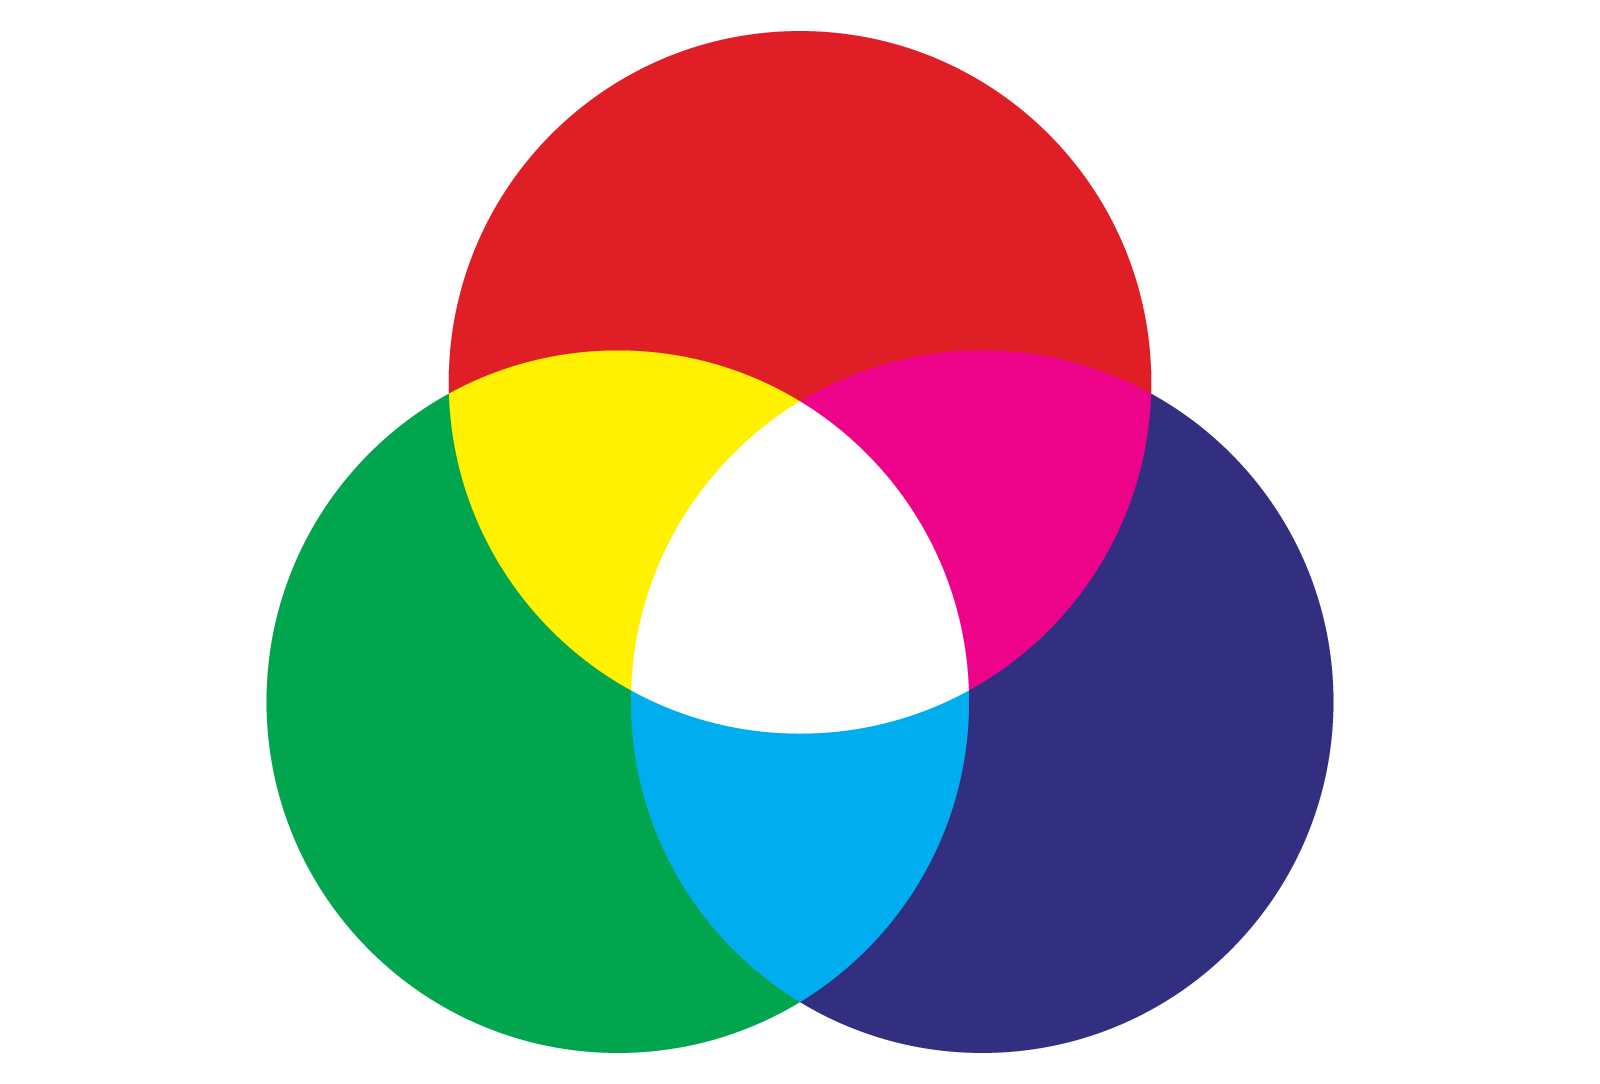
\includegraphics[width=\textwidth]{images/cover.png}
        \vfill

        \hrule
        \begin{minipage}{0.495\textwidth} 
            \vspace{0.4em}
            \raggedright
            \normalsize 
            Name: \censor{Andrew Hayes} \\
            E-mail: \censor{\href{mailto://a.hayes18@universityofgalway.ie}{\texttt{a.hayes18@universityofgalway.ie}}}  \hfill\\   
            Student ID: \censor{21321503} \hfill
        \end{minipage}
        \begin{minipage}{0.495\textwidth} 
            \raggedleft
            \vspace*{0.8cm}
            \Large
            \today
            \vspace*{0.6cm}
        \end{minipage}
        \medskip\hrule 
    \end{center}
\end{titlepage}

\pagenumbering{roman}
\newpage
\tableofcontents
\newpage
\setcounter{page}{1}
\pagenumbering{arabic}

\section{Introduction}
Textbooks:
\begin{itemize}
    \item   Main textbook: \textit{Image Processing and Analysis} -- Stan Birchfield (ISBN: 978-1285179520).
    \item   \textit{Introduction to Computer Graphics} -- David J. Eck. (Available online at \url{https://math.hws.edu/graphicsbook/}).
    \item   \textit{Computer Graphics: Principles and Practice} -- John F. Hughes et al. (ISBN: 0-321-39952-8).
    \item   \textit{Computer Vision: Algorithms and Applications} -- Richard Szeliski (ISBN: 978-3-030-34371-2).
\end{itemize}

\textbf{Computer graphics} is the processing \& displaying of images of objects that exist conceptually rather than
physically with emphasis on the generation of an image from a model of the objects, illumination, etc. and the
real-time rendering of images.
Ideas from 2D graphics extend to 3D graphics.
\\\\
\textbf{Digital Image processing/analysis} is the processing \& display of images of real objects, with an emphasis
on the modification and/or analysis of the image in order to automatically or semi-automatically extract useful
information.
Image processing leads to more advanced feature extraction \& pattern recognition techniques for image analysis \&
understanding.

\subsection{Grading}
\begin{itemize}
    \item   Assignments: 30\%.
    \item   Final Exam: 70\%.
\end{itemize}

\subsubsection{Reflection on Exams}
``A lot of people give far too little detail in these questions, and/or don't address the discussion 
parts -- they just give some high-level definitions and consider it done -- which isn't enough for 
final year undergrad, and isn't answering the question.
More is expected in answers than just repeating what's in my slides. 
The top performers demonstrate a higher level of understanding and synthesis as well as more 
detail about techniques and discussion of what they do on a technical level and how they fit 
together''

\subsection{Lecturer Contact Information}
\begin{multicols}{2}
    \begin{itemize}
        \item   Dr. Nazre Batool.
        \item   \href{mailto://nazre.batool@universityofgalway.ie}{\texttt{nazre.batool@universityofgalway.ie}}
        \item   Office Hours: Thursdays 16:00 -- 17:00, CSB-2009.

        \item   Dr. Waqar Shahid Qureshi.
        \item   \href{mailto://waqarshahid.qureshi@universityofgalway.ie}{\texttt{waqarshahid.qureshi@universityofgalway.ie}}.
        \item   Office Hours: Thursdays 16:00 -- 17:00, CSB-3001.
    \end{itemize}
\end{multicols}

\section{Introduction to 2D Graphics}
\subsection{Digital Images -- Bitmaps}
\textbf{Bitmaps} are grid-based arrays of colour or brightness (greyscale) information.
\textbf{Pixels} (\textit{picture elements}) are the cells of a bitmap.
The \textbf{depth} of a bitmap is the number of bits-per-pixel (bpp).

\subsection{Colour Encoding Schemes}
Colour is most commonly represented using the \textbf{RGB (Red, Green, Blue)} scheme, typically using 24-bit colour
with one 8-bit number representing the level of each colour channel in that pixel.
\\\\
Alternatively, images can also be represented in \textbf{greyscale} wherein pixels are represented with one
(typically 8-bit) brightness value (or scale of grey) .

\subsection{The Real-Time Graphics Pipeline}
\begin{figure}[H]
    \centering
    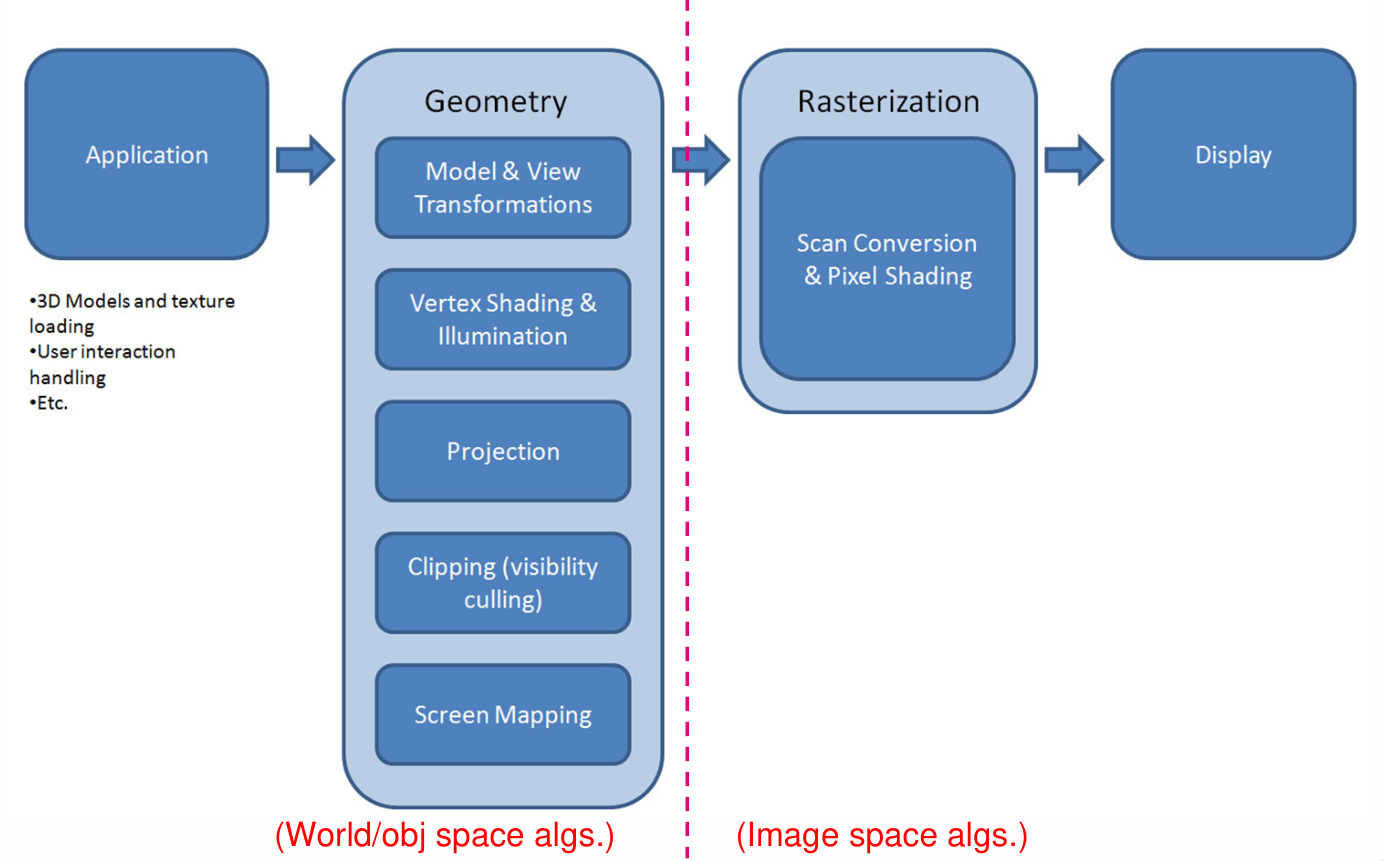
\includegraphics[width=\textwidth]{images/real_time_graphics_pipeline.png}
    \caption{The Real-Time Graphics Pipeline}
\end{figure}

\subsection{Graphics Software}
The \textbf{Graphics Processing Unit (GPU)} of a computer is a hardware unit designed for digital image processing \& to 
accelerate computer graphics that is included in modern computers to complement the CPU.
They have internal, rapid-access GPU memory and parallel processors for vertices \& fragments to speed up graphics 
renderings.
\\\\
\textbf{OpenGL} is a 2D \& 3D graphics API that has existed since 1992 that is supported by the graphics hardware in most
computing devices today.
\textbf{WebGL} is a web-based implementation of OpenGL for use within web browsers.
OpenGL ES for Embedded Systems such as tablets \& mobile phones also exists.
\\\\
OpenGL was originally a client/server system with the CPU+Application acting as a client sending commands \& data to the GPU
acting as a server.
This was later replaced by a programmable graphics interface (OpenGL 3.0) to write GPU programs (shaders) to be run by the 
GPU directly.
It is being replaced by newer APIs such as Vulkan, Metal, \& Direct3D and WebGL is being replaced by WebGPU.

\subsection{Graphics Formats}
\textbf{Vector graphics} are images described in terms of co-ordinate drawing operations, e.g. AutoCAD, PowerPoint, Flash, 
SVG.
\textbf{SVG (Scalable Vector Graphics)} is an image specified by vectors which are scalable without losing any quality.
\\\\
\textbf{Raster graphics} are images described as pixel-based bitmaps.
File formats such as GIF, PNG, JPEG represent the image by storing colour values for each pixel.

\section{2D Vector Graphics}
\textbf{2D vector graphics} describe drawings as a series of instructions related to a 2-dimensional co-ordinate system.
Any point in this co-ordinate system can be specified using two numbers $(x, y)$:
\begin{itemize}
    \item   The horizontal component $x$, measuring the distance from the left-hand edge of the screen or window.
    \item   The vertical component $y$, measuring the distance from the bottom of the screen or window (or sometimes from the
            top).
\end{itemize}

\subsection{Transformations}
\subsubsection{2D Translation}
The \textbf{translation} of a point in 2 dimensions is the movement of a point $(x,y)$ to some other point $(x', y')$.
$$
x' = x + a
$$
$$
y' = y + b
$$

\begin{figure}[H]
    \centering
    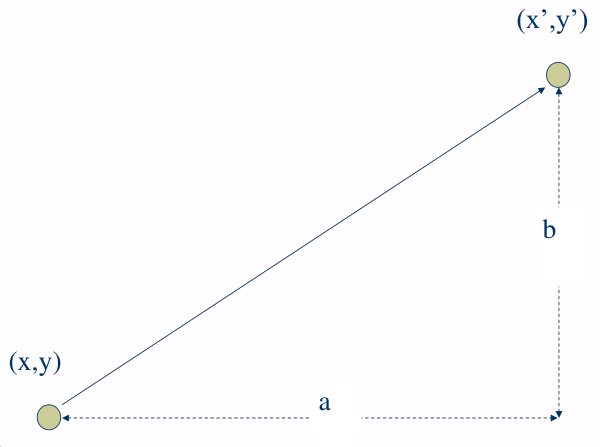
\includegraphics[width=0.5\textwidth]{images/2d_translation.png}
    \caption{2D Translation of a Point}
\end{figure}

\subsubsection{2D Rotation of a \textit{Point}}
The simplest rotation of a point around the origin is given by:
$$
x' = x \cos \theta - y \sin \theta
$$
$$
y' = x \cos \theta + y \sin \theta
$$

\begin{figure}[H]
    \centering
    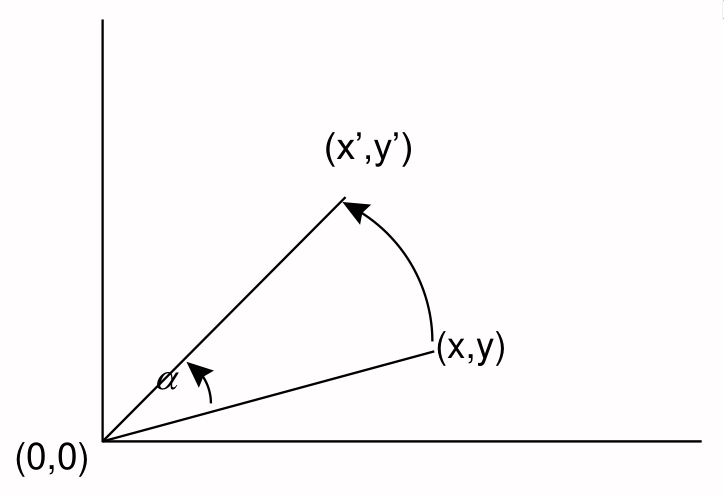
\includegraphics[width=0.5\textwidth]{images/2d_point_rotation.png}
    \caption{2D Rotation of a Point}
\end{figure}

\subsubsection{2D Rotation of an \textit{Object}}
In vector graphics, \textbf{objects} are defined as series of drawing operations (e.g., straight lines) performed on a set 
of vertices.
To rotate a line or more complex object, we simply apply the equations to rotate a point to the $(x,y)$ co-ordinates of each 
vertex.

\begin{figure}[H]
    \centering
    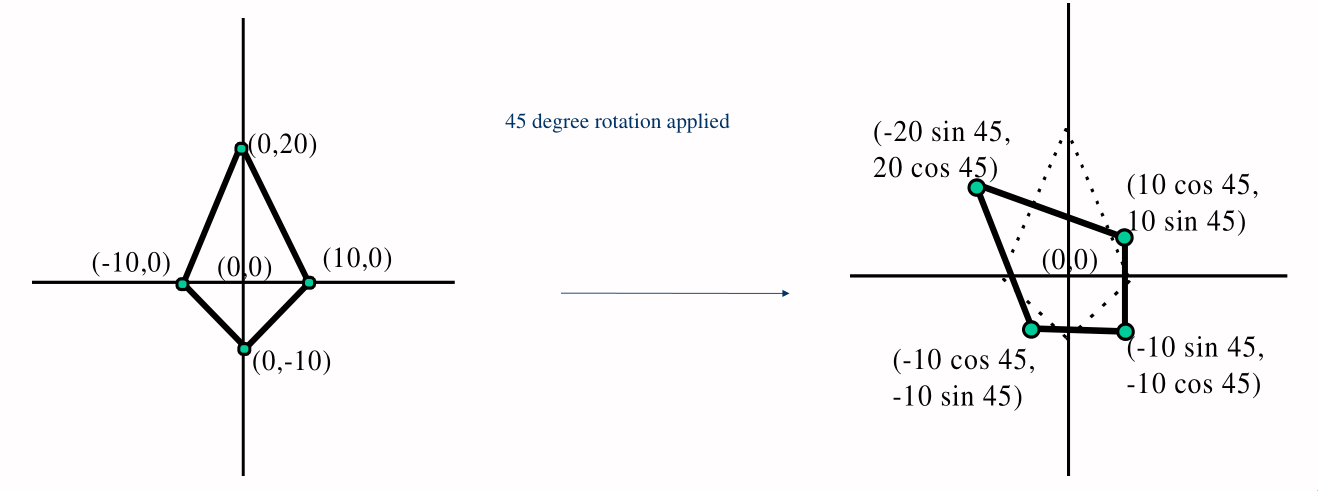
\includegraphics[width=0.7\textwidth]{images/2d_object_rotation.png}
    \caption{2D Rotation of an Object}
\end{figure}

\subsubsection{Arbitrary 2D Rotation}
In order to rotate around an arbitrary point $(a,b)$, we perform translation, then rotation, then reverse the translation.
$$
x' = a + (x - a) \cos \theta - (y - b) \sin \theta
$$
$$
y' = a + (x - a) \cos \theta + (y - b) \sin \theta
$$

\begin{figure}[H]
    \centering
    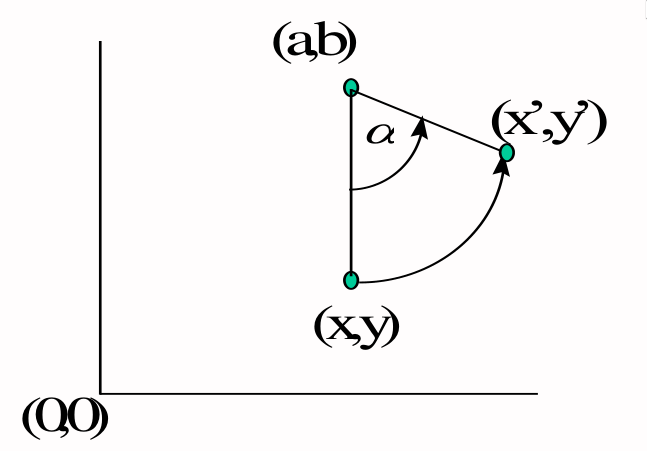
\includegraphics[width=0.5\textwidth]{images/2d_arbitrary_rotation.png}
    \caption{Arbitrary 2D Rotation}
\end{figure}

\subsubsection{Matrix Notation}
\textbf{Matrix notation} is commonly used for vector graphics as more complex operations are often easier in matrix format 
and because several operations can be combined easily into one matrix using matrix algebra.

Rotation about $(0,0)$:
$$
\begin{bmatrix}
    x' & y'
\end{bmatrix}
=
\begin{bmatrix}
    x & y
\end{bmatrix}
\begin{bmatrix}
 \cos \theta & \sin \theta \\
-\sin \theta & \cos \theta
\end{bmatrix}
$$

Translation:
$$
\begin{bmatrix}
    x' & y' 1
\end{bmatrix}
=
\begin{bmatrix}
    x & y & 1
\end{bmatrix}
\begin{bmatrix}
    1 & 0 & 0 \\
    0 & 1 & 0 \\
    a & 0 & 1
\end{bmatrix}
$$

\subsubsection{Scaling}
\textbf{Scaling} of an object is achieved by considering each of its vertices in turn, multiplying said vertex's $x$ \& $y$
values by the scaling factor.
A scaling factor of 2 will double the size of the object, while a scaling factor of 0.5 will halve it.
It is possible to have different scaling factors for $x$ \& $y$, resulting in a \textbf{stretch}:
$$
x' = x \times s
$$
$$
y' = y \times t
$$

If the object is not centred on the origin, then scaling it will also effect a translation.

\subsubsection{Order of Transformations}
\begin{figure}[H]
    \centering
    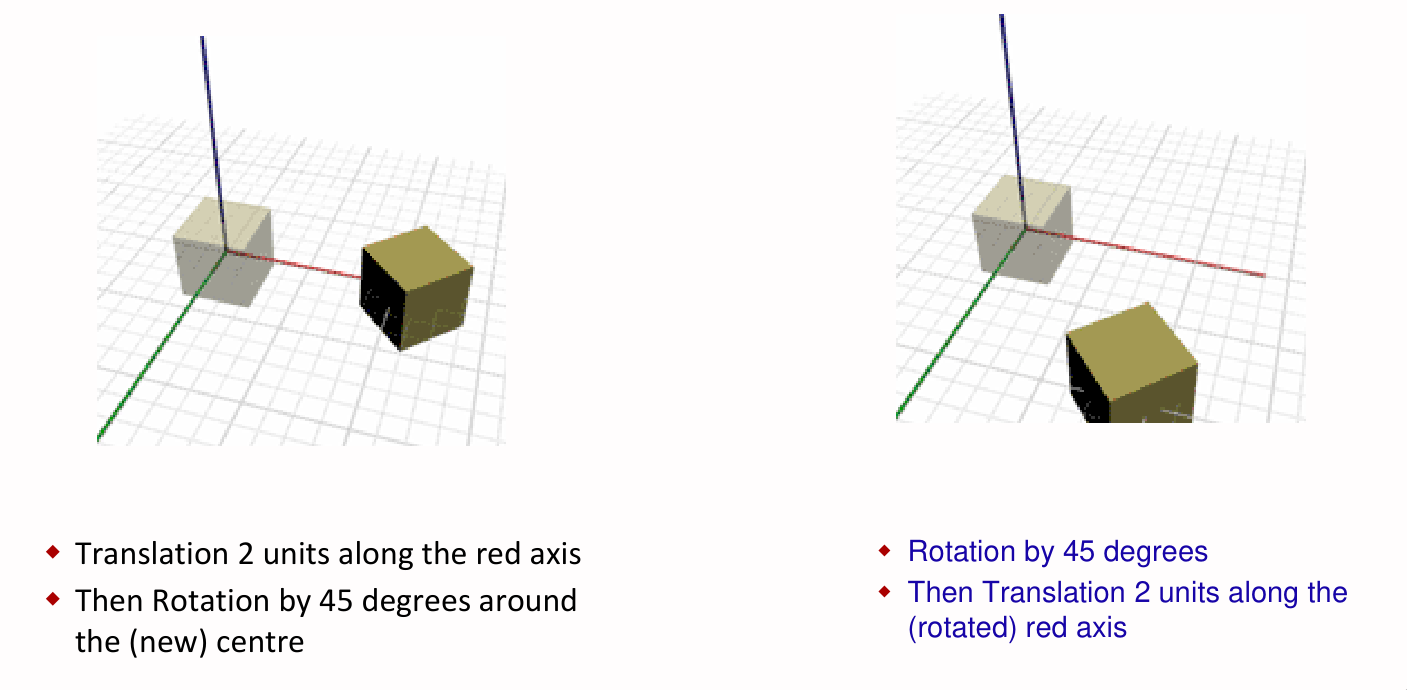
\includegraphics[width=0.8\textwidth]{images/order_of_transformations.png}
    \caption{Order of Transformations}
\end{figure}

\section{2D Raster Graphics}
The raster approach to 2D graphics considers digital images to be grid-based arrays of pixels and operates on the 
images at the pixel level.

\subsection{Introduction to HTML5/Canvas}
\textbf{HTML} or HyperText Markup Language is a page-description language used primarily for website.
\textbf{HTML5} brings major updates \& improvements to the power of client-side web development.
\\\\
A \textbf{canvas} is a 2D raster graphics component in HTML5.
There is also a \textbf{canvas with 3D} (WebGL) which is a 3D graphics component that is more likely to be 
hardware-accelerated but is also more complex.

\subsubsection{Canvas: Rendering Contexts}
\mintinline{html}{<canvas>} creates a fixed-size drawing surface that exposes one or more \textbf{rendering contexts}.
The \mintinline{javascript}{getContext()} method returns an object with tools (methods) for drawing.

\begin{minted}[linenos, breaklines, frame=single]{html}
<html>
    <head>
        <script>
            function draw() {
                var canvas = document.getElementById("canvas");
                var ctx = canvas.getContext("2d");
                ctx.fillStyle = "rgb(200,0,0)";
                ctx.fillRect (10, 10, 55, 50);
                ctx.fillStyle = "rgba(0, 0, 200, 0.5)";
                ctx.fillRect (30, 30, 55, 50);
            }
        </script>
    </head>
    <body onload="draw();">
        <canvas id="canvas" width="150" height="150"></canvas>
    </body>
</html>
\end{minted}

\begin{figure}[H]
    \centering
    
\includegraphics[width=0.2\textwidth]{images/canvas_rendering_contexts.png}
    \caption{Rendering of the Above HTML Code}
\end{figure}

\subsubsection{Canvas2D: Primitives}
Canvas2D only supports one primitive shape: rectangles.
All other shapes must be created by combining one or more \textit{paths}.
Fortunately, there are a collection of path-drawing functions which make it possible to compose complex shapes.

\begin{minted}[linenos, breaklines, frame=single]{javascript}
function draw(){
    var canvas = document.getElementById('canvas');
    var ctx = canvas.getContext('2d');
    ctx.fillRect(125,25,100,100);
    ctx.clearRect(145,45,60,60);
    ctx.strokeRect(150,50,50,50);
    ctx.beginPath();
    ctx.arc(75,75,50,0,Math.PI*2,true); // Outer circle
    ctx.moveTo(110,75);
    ctx.arc(75,75,35,0,Math.PI,false);   // Mouth (clockwise)
    ctx.moveTo(65,65);
    ctx.arc(60,65,5,0,Math.PI*2,true);  // Left eye
    ctx.moveTo(95,65);
    ctx.arc(90,65,5,0,Math.PI*2,true);  // Right eye
    ctx.stroke(); // renders the Path that has been built up..
}
\end{minted}

\begin{figure}[H]
    \centering
    
\includegraphics[width=0.3\textwidth]{images/canvas2d_primitives.png}
    \caption{Rendering of the Above JavaScript Code}
\end{figure}

\subsubsection{Canvas2D: \mintinline{javascript}{drawImage()}}
The example below uses an external image as the backdrop of a small line graph:
\begin{minted}[linenos, breaklines, frame=single]{javascript}
function draw() {
    var ctx = document.getElementById('canvas').getContext('2d');
    var img = new Image();
    img.src = 'backdrop.png';
    img.onload = function(){
        ctx.drawImage(img,0,0);
        ctx.beginPath();
        ctx.moveTo(30,96);
        ctx.lineTo(70,66);
        ctx.lineTo(103,76);
        ctx.lineTo(170,15);
        ctx.stroke();
    }
}
\end{minted}

\begin{figure}[H]
    \centering
    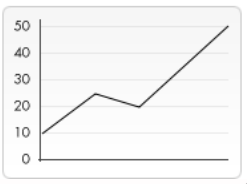
\includegraphics[width=0.3\textwidth]{images/canvas2d_drawimage.png}
    \caption{Rendering of the Above JavaScript Code}
\end{figure}

\subsubsection{Canvas2D: Fill \& Stroke Colours}
\begin{minted}[linenos, breaklines, frame=single]{html}
<html>
    <head>
        <script>
            function draw() {
                var canvas = document.getElementById("canvas");
                var context = canvas.getContext('2d');
                // Filled Star
                context.lineWidth=3;
                context.fillStyle="#CC00FF";
                context.strokeStyle="#ffff00"; // NOT lineStyle!
                context.beginPath();
                context.moveTo(100,50);
                context.lineTo(175,200);
                context.lineTo(0,100);
                context.lineTo(200,100);
                context.lineTo(25,200);
                context.lineTo(100,50);
                context.fill(); // colour the interior
                context.stroke(); // draw the lines
            }
        </script>
    </head>
    <body onload="draw();">
        <canvas id="canvas" width="300" height="300"></canvas>
    </body>
</html>
\end{minted}

Colours can be specified by name (\mintinline{javascript}{red}), by a string of the form
\mintinline{javascript}{rgb(r,g,b)}, or by hexadecimal colour codes \mintinline[escapeinside=||]{javascript}{|#|RRGGBB}.

\begin{figure}[H]
    \centering
    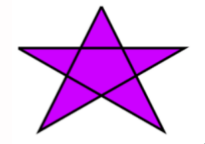
\includegraphics[width=0.3\textwidth]{images/canvas2d_fill_stroke.png}
    \caption{Rendering of the Above JavaScript Code}
\end{figure}

\subsubsection{Canvas2D: Translations}
\begin{minted}[linenos, breaklines, frame=single]{html}
<html>
    <head>
        <script>
            function draw() {
                var canvas = document.getElementById("canvas");
                var context = canvas.getContext('2d');
                context.save(); // save the default (root) co-ord system
                context.fillStyle="#CC00FF"; // purple
                context.fillRect(100,0,100,100);
                // translates from the origin, producing a nested co-ordinate system
                context.translate(75,50);
                context.fillStyle="#FFFF00"; // yellow
                context.fillRect(100,0,100,100);
                // transforms further, to produce another nested co-ordinate system
                context.translate(75,50);
                context.fillStyle="#0000FF"; // blue
                context.fillRect(100,0,100,100);
                context.restore(); // recover the default (root) co-ordinate system
                context.translate(-75,90);
                context.fillStyle="#00FF00"; // green
                context.fillRect(100,0,100,100);
            }
        </script>
    </head>
    <body onload="draw();">
        <canvas id="canvas" width="600" height="600"></canvas>
    </body>
</html>
\end{minted}

\begin{figure}[H]
    \centering
    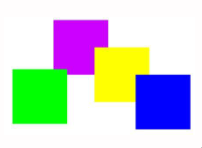
\includegraphics[width=0.3\textwidth]{images/canvas2d_translations.png}
    \caption{Rendering of the Above JavaScript Code}
\end{figure}

\subsubsection{Canvas2D: Order of Transformations}
\begin{minted}[linenos, breaklines, frame=single]{html}
<html>
    <head>
        <script>
            function draw() {
                var canvas = document.getElementById("canvas");
                var context = canvas.getContext('2d');
                context.save(); // save the default (root) co-ord system
                context.fillStyle="#CC00FF"; // purple
                context.fillRect(0,0,100,100); // positioned with TL corner at 0,0
                // translate then rotate
                context.translate(100,0);
                context.rotate(Math.PI/3);
                context.fillStyle="#FF0000"; // red
                context.fillRect(0,0,100,100); // positioned with TL corner at 0,0
                // recover the root co-ord system
                context.restore();
                // rotate then translate
                context.rotate(Math.PI/3);
                context.translate(100,0);
                context.fillStyle="#FFFF00"; // yellow
                context.fillRect(0,0,100,100); // positioned with TL corner at 0,0
            }
        </script>
    </head>
    <body onload="draw();">
        <canvas id="canvas" width="600" height="600"></canvas>
    </body>
</html>
\end{minted}

\begin{figure}[H]
    \centering
    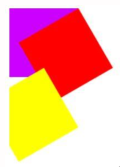
\includegraphics[width=0.2\textwidth]{images/canvas2d_order_of_transformations.png}
    \caption{Rendering of the Above JavaScript Code}
\end{figure}

\subsubsection{Scaling}
\begin{minted}[linenos, breaklines, frame=single]{html}
<html>
    <head>
        <script>
            function draw() {
                var canvas = document.getElementById("canvas");
                var context = canvas.getContext('2d');
                context.fillStyle="#CC00FF"; // purple
                context.fillRect(0,0,100,100); // positioned with TL corner at 0,0
                context.translate(150,0);
                context.scale(2,1.5);
                context.fillStyle="#FF0000"; // red
                context.fillRect(0,0,100,100); // positioned with TL corner at 0,0
            }
        </script>
    </head>
    <body onload="draw();">
        <canvas id="canvas" width="600" height="600"></canvas>
    </body>
</html>
\end{minted}

\begin{figure}[H]
    \centering
    
\includegraphics[width=0.2\textwidth]{images/canvas2d_scaling.png}
    \caption{Rendering of the Above JavaScript Code}
\end{figure}

\subsubsection{Canvas2D: Programmatic Graphics}
\begin{minted}[linenos, breaklines, frame=single]{html}
<html>
    <head>
        <script>
            function draw() {
                var canvas = document.getElementById("canvas");
                var context = canvas.getContext('2d');
                context.translate(150,150);
                for (i=0;i<15;i++) {
                    context.fillStyle = "rgb("+(i*255/15)+",0,0)";
                    context.fillRect(0,0,100,100);
                    context.rotate(2*Math.PI/15);
                }
            }
        </script>
    </head>
    <body onload="draw();">
        <canvas id="canvas" width="600" height="600"></canvas>
    </body>
</html>
\end{minted}

\begin{figure}[H]
    \centering
    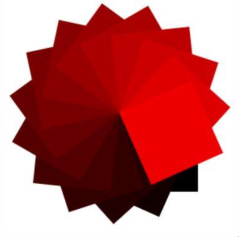
\includegraphics[width=0.2\textwidth]{images/canvas2d_programmatic_graphics.png}
    \caption{Rendering of the Above JavaScript Code}
\end{figure}


\end{document}
